\section{Seuillage}
\begin{enumerate}
  \item \q{A partir des fourchettes établies précédemment, transformer
          l’image en noir et blanc ou seule la voiture sera blanche.}\\
        Toujours pour l'impression, j'ai fait l'inverse au niveau des couleurs :
        \codeFromFileT{helpers/image.py}{section-03/q1-1.py}
        \codeFromFileT{main.py}{section-03/q1-2.py}
        J'obtiens alors :
        \begin{center}
          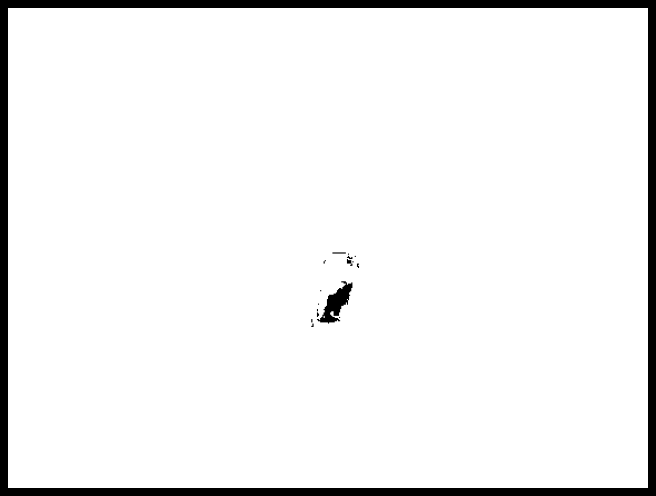
\includegraphics[scale=0.2]{section-03/q1-3.py}
        \end{center}
\end{enumerate}
